\documentclass{article}
\usepackage[margin = 0.15in,landscape]{geometry}
\usepackage{multicol}
\usepackage{array}
\usepackage{amsmath}
\usepackage{amssymb}
\usepackage{lmodern}
\usepackage{graphicx}
\usepackage{enumitem}
\setlength\parindent{0pt}
%\renewcommand{\baselinestretch}{0.75}


\begin{document}
\begin{multicols}{3}
    Marissa Palamara\par 
    ASEN 3112\par 
    Spring 2021
    %\vspace{-0.2cm}
    \setlist{nolistsep}
    % ----- Introduction to Second Law ----- %
    \section*{2nd Law}
    \textbf{The Second Law of Thermodynamics}: Processes occur in a certain direction and energy has quality as well as quantity.\par
    \textbf{Thermal Energy Reservoirs}: A hypothetical body with a relatively large thermal energy capacity (mass x specific heat) that can supply or absorb finite amounts of heat without undergoing any change in temperature. 
    % Heat Engines
    \subsection*{Heat Engines}
    \begin{itemize}
        \item Devices that convert heat to work
        \item Receive heat from high-temp source
        \item Convert part of this heat to work
        \item Reject remaining waste heat to low-temperature sink - Kelvin-Plank Statement
        \item Operate on a cycle
        \item MUST waste some energy by transferring to low-temperature reservoir in order to complete cycle
    \end{itemize}
    Notation:
    \begin{itemize}
        \item $Q_{in}=Q_H$ = amount of heat supplied from a high-temp source
        \item $Q_{out}=Q_L$ = amount of heat rejected to a low temperature sink
        \item $W_{out}$ = amount of work delivered out of system by working fluid
        \item $W_{in}$ = amount of work input to system
    \end{itemize}
    $W_{net,out}=W_{out}-W_{in}\text{ (kJ)}$\par 
    $W_{net,out}=Q_{in}-Q_{out}\text{ (kJ)}$
    % Thermal Efficiency
    \subsection*{Thermal Efficiency}
    $\eta = \frac{W_{net,out}}{Q_{in}}=1-\frac{Q_{out}}{Q_{in}}=1-\frac{Q_L}{Q_H}$
    % Refrigerators and Heat Pumps
    \subsection*{Refrigerators and Heat Pumps}
    \textbf{Coefficient of Performance}: efficiency of a refrigerator.\par 
    $\text{COP}_R=\frac{\text{Desired Output}}{\text{Required Input}}=\frac{Q_L}{W_{net,in}}=\frac{Q_L}{Q_H-Q_L}=\frac{1}{Q_H/Q_L-1}$ \par 
    \textbf{Clausius Statement}: It is impossible to construct a device that operates in a cycle and produces no effect other than the transfer of heat from a lower-temperature body to a higher-temperature body.\par
    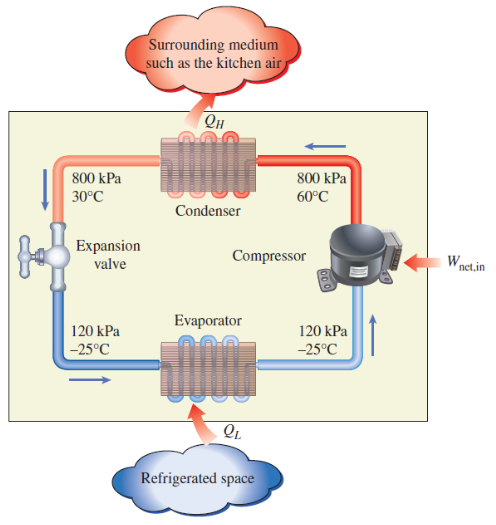
\includegraphics[width=0.75\linewidth]{Images/refrigerator.png}
    \subsection*{Reversible and Irreversible Processes}
    \textbf{Reversible Process}: A process that can be reversed without leaving any trace on the surroundings - theoretical to find limits.\par 
    \textbf{Irreversible Process}: A process that is not reversible.\par 
    \textbf{Ierreversibilities}:
    \begin{itemize}
        \item Friction
        \item Unrestrained expansion
        \item Mixing of two fluids
        \item Heat transfer across a finite temperature difference
        \item Electric resistance
        \item Inelastic deformation of solids
        \item Chemical reactions
    \end{itemize}
    % The Carnot Cycle
    \subsection*{The Carnot Cycle}
    The Carnot Cycle is composed of four reversible processes - two isothermal and two adiabatic - and it can be executed either in a closed or steady-flow system.
    \begin{itemize}
        \item Reversible Isothermal Expansion - \\process 1-2, $T_H$ = constant
        \item Reversible Adiabatic Expansion - \\process 2-3, $T_H\rightarrow T_L$
        \item Reversible Isothermal Compression - \\process 3-4, $T_L$ = constant
        \item Reversible Adiabtic Compression - \\process 4-1, $T_L\rightarrow T_H$
    \end{itemize}
    The Carnot Cycle is completely reversible - in which case it becomes the carnot refrigeration cycle.\par
    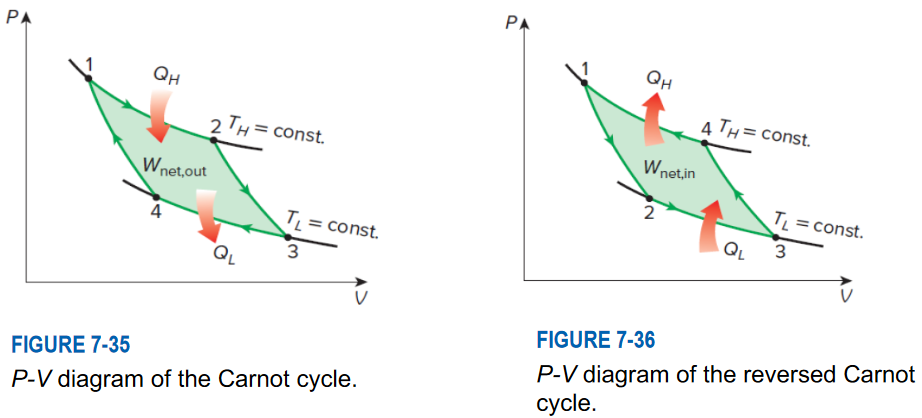
\includegraphics[width=\linewidth]{Images/Pv_Carnot.png}
    \textbf{The Carnot Principles}: The efficiency of an irreversible heat engine is always less than the efficiency of a reversible one operating between the same two reservoirs and the efficiencies of all reversible heat engines operating between the same two reservoirs are the same.\par
    \textbf{The Thermodynamic Temperature Scale}: A temperature scale that is independent of the properties of the substances that are used to measure temperature.\par 
    $T_H=T_L\frac{Q_H}{Q_L}$\par 
    % The Carnot Heat Engine
    \subsection*{The Carnot Heat Engine}
    Any heat engine: $\eta_{th}=1-\frac{Q_L}{Q_H}$\par 
    Carnot heat engine: $\eta_{th,rev}=1-\frac{T_L}{T_H}$\par 
    \begin{equation*}
        \eta_{th}\left\{
            \begin{array}{l}
                <\eta_{th,rev}\text{ irreversible heat engine}\\
                =\eta_{th,rev}\text{ reversible heat engine}\\
                >\eta_{th,rev}\text{ impossible heat engine}
            \end{array}
        \right.
    \end{equation*}
    Amount of heat rejected per cycle: $Q_{L,rev}=\frac{T_L}{T_H}Q_{H,rev}$\par 
    \textbf{Quality of Energy}: The higher the temperature of the thermal energy, the higher its quality. Directly relates to face that you can use temperature to measure efficiency in $\eta_{th,rev}$.
    % The Carnot Refrigerator and Heat Pump
    \subsection*{The Carnot Refrigerator and Heat Pump}
    Any refrigerator or heat pump:\par 
    $\text{COP}_R=\frac{1}{Q_H/Q_L-1}$ and $\text{COP}_{HP}=\frac{1}{1-Q_L/Q_H}$\par 
    Carnot refrigerator or heat pump:\par 
    $\text{COP}_{R,rev}=\frac{1}{T_H/T_L-1}$ and $\text{COP}_{HP,rev}=\frac{1}{1-T_L/T_H}$
    \begin{equation*}
        \text{COP}_{R}\left\{
            \begin{array}{l}
                <\text{COP}_{R,rev}\text{ irreversible refrigerator}\\
                =\text{COP}_{R,rev}\text{ reversible refrigerator}\\
                >\text{COP}_{R,rev}\text{ impossible refrigerator}
            \end{array}
        \right.
    \end{equation*}
    
    % ----- Entropy ----- %
    \newpage
    \section*{Entropy}
    \begin{itemize}
        \item Processes can only occur in a certain direction and that direction must comply with the increase of entropy principle: $S_\text{gen}\geq 0$.
        \item Entropy is a nonconserved property, and there is no such thing as the conservation of entropy principle. Entropy is conserved during the idealized reversible processes only and increases during all actual processes.
        \item Entropy generation is the measure of the magnitudes of the irreversibilities during the performance of engineering systems. It is also used to establish criteria for the performance of engineering devices.
    \end{itemize}
    \textbf{Clausius Inequality}: \fbox{$\oint\frac{\delta Q}{T}\leq 0$}\par 
    $\delta W_C=\delta Q_R-dE_C$\par 
    Reversible cyclic device:\par $\frac{\delta Q_R}{T_R}=\frac{\delta Q}{T}\rightarrow \delta W_C=T_R\frac{\delta Q}{T}-dE_C$\par 
    For a system underoing a cycle: $W_C=T_R\oint\frac{\delta Q}{T}$\par 
    $\oint\left(\frac{\delta Q}{T}\right)_\text{{int,rev}}=0$ and $dS=\left(\frac{\delta Q}{T}\right)_{\text{int,rev}}$ (kJ/K)\par
    \textbf{Entropy}: $\Delta S=S_2-S_1=\int_1^2\left(\frac{\delta Q}{T}\right)_{\text{int,rev}}$\par
    \textbf{Special Case}: \par Internally Reversible Isothermal Heat Transfer Process $\Delta S=\frac{Q}{T_0}$ (kJ/K) where $T_0$ is the constant temperature of the system and $Q$ is the heat transfer for the internally reversible process.\par 
    \textbf{Generated Entropy}: \par
    $S_{\text{gen}}=\Delta S_{\text{total}}=\Delta S_{\text{sys}}+\Delta S_{\text{surr}}\geq 0\rightarrow \Delta S_{\text{sys}}=S_2-S_1=\int_1^2\frac{\delta Q}{T}+S_\text{gen}$\par 
    \textbf{The Increase of Entropy Principle}:
    \begin{equation*}
        S_\text{gen}\left\{
            \begin{array}{l}
                <0\text{ impossible process}\\
                =0\text{ reversible process}\\
                >0\text{ irreversible process}
            \end{array}
        \right.
    \end{equation*}
    % Entropy Change of Pure Substances
    \subsection*{Entropy Change of Pure Substances}
    Once the state of the system is fixed the value of entropy is also fixed.\par 
    $\Delta S=m\Delta s=m(s_2-s_1)$ (kJ/K)\par
    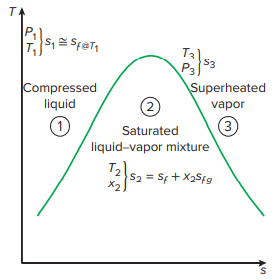
\includegraphics[width=0.5\linewidth]{Images/entropy_pure_subtances.png}\par 
    T-s Diagram for water$\downarrow$\par
    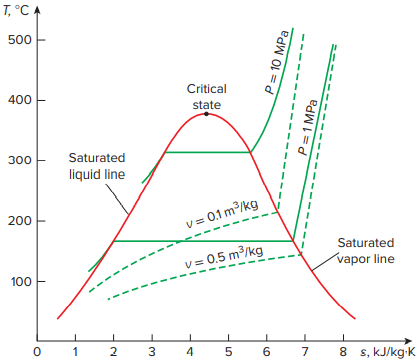
\includegraphics[width=0.5\linewidth]{Images/Ts_water.png}
    % Isentropic Processes
    \subsection*{Isentropic Processes}
    $\Delta S=0$ or $S_2=S_1$ (kJ/kgK)
    % Property Diagrams
    \subsection*{Property Diagrams involving Entropy}
    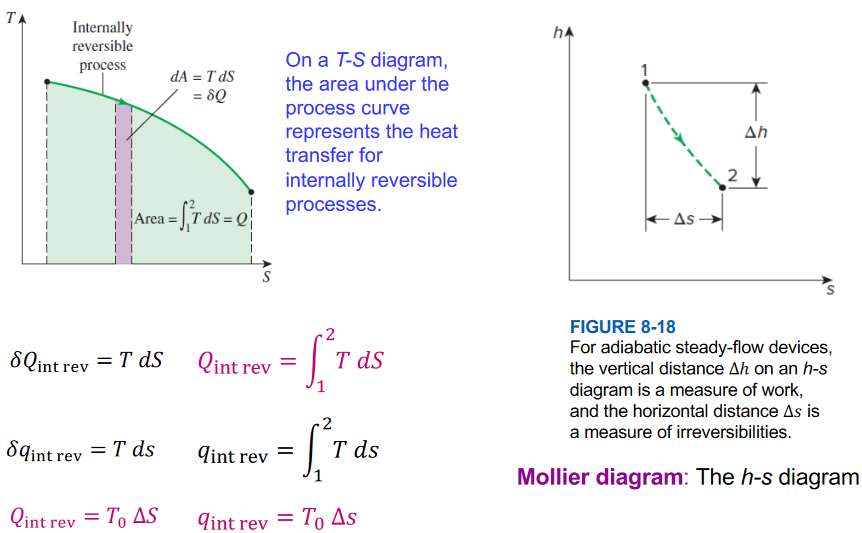
\includegraphics[width=\linewidth]{Images/Diagrams1.png}\par 
    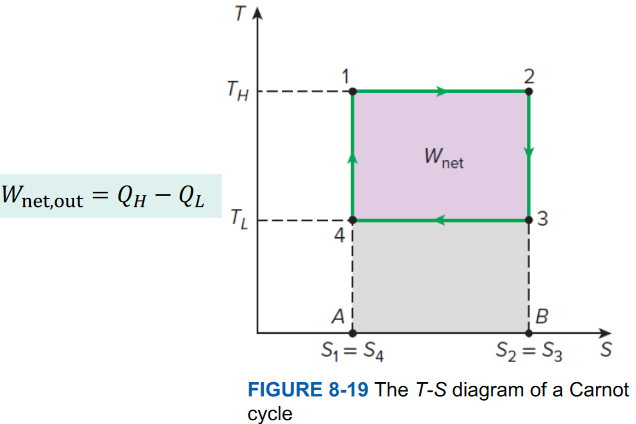
\includegraphics[width=0.5\linewidth]{Images/Diagrams2.png}
    % What is Entropy
    \subsection*{What is Entropy?}
    \textbf{Boltzmann Relation}: $S=k\ln{W}$\par 
    $k=1.3806\times 10^{-23}$ J/K\par 
    \textbf{Gibb's Formulation}: $S=-k\sum P_i\log{P_i}$\par 
    \textbf{Pure Crystal}: $T=0$ K then Entropy = 0\par The entropy of a pure crystalline substance at absolute zero temperature is zero (Third Law of Thermodynamics)
    % The Tds Relations
    \subsection*{The $Tds$ Relations}
    \textbf{The First $Tds$ or Gibbs Equation}:\par 
    $\delta Q_\text{int,rev}-\delta W_\text{int,rev,out}=dU$\par 
    $\delta Q_\text{int,rev}=TdS$ and $\delta W_\text{int rev,out}=PdV$\par 
    $TdS=dU+PdV$ (kJ)\par 
    \fbox{$Tds=du+Pdv$}\par 
    \textbf{The Second $Tds$ Equation}:\par 
    $h=u+Pv$\par 
    $dh=du+Pdv+vdP$ and $Tds=du+Pdv$\par 
    \fbox{$Tds=dh-vdP$}\par 
    \textbf{Finally}:\par 
    \fbox{$ds=\frac{du}{T}+\frac{Pdv}{T}=\frac{dh}{T}-\frac{vdP}{T}$}
    % Entropy Change of Liquids and Solids
    \subsection*{Entropy Change of Liquids and Solids}
    Liquids and solids can be approximated as incompressible substances $\rightarrow dv=0$.\par 
    $ds=\frac{du}{T}=\frac{cdT}{T}\rightarrow c_P=c_v=c\text{ and }du=cdT$\par 
    \fbox{$S_2-S_1=\int_1^2d(T)\frac{dT}{T}=c_\text{avg}\ln{\frac{T_2}{T_1}}$ (kJ/kgK)}\par 
    Isentropic: $s_2-s_1=c_\text{avg}\ln{\frac{T_2}{T_1}}=0\rightarrow T_2=T_1$
    % Entropy Change of Ideal Gases
    \subsection*{Entropy Change of Ideal Gases}
    $Pv=RT$\par 
    $du=c_vdT$\par 
    $dh=c_pdT$\par 
    $ds=c_v\frac{dT}{T}+R\frac{dv}{v}\rightarrow s_2-s_1=\int_1^2c_v(T)\frac{dT}{T}+R\ln{\frac{v_2}{v_1}}$\par
    $s_2-s_1=\int_1^2c_p(T)\frac{dT}{T-R\ln{\frac{P_2}{P_1}}}$
    % Constant Specific Heats
    \subsection*{Constant Specific Heats (Approximate Analysis)}
    $s_2-s_1=c_{v,avg}\ln\frac{T_2}{T_1}+R\ln\frac{v_2}{v_1}$\par 
    $s_2-s_1=c_{p,avg}\ln\frac{T_2}{T_1}-R\ln\frac{P_2}{P_1}$
    \subsection*{Variable Specific Heats (Exact Analysis)}
    $s_2-s_1=\int_1^2c_v(T)\frac{dT}{T}+R\ln{\frac{v_2}{v_1}}$\par 
    Choose absolute zero as reference temperature and define a function $s^\circ$ as:\par 
    $s^\circ=int_0^Tc_p(T)\frac{dT}{T}$\par 
    $s_2^\circ-s_1^\circ=\int_1^2c_p(T)\frac{dT}{T}$\par 
    On a unit mass basis: \par 
    $s_2-s_1=s_2^\circ-s_1^\circ-R\ln\frac{P_2}{P_1}\text{ (kJ/kgK)}$\par 
    % Isentropic Processes of Ideal Gases
    \subsection*{Isentropic Processes of Ideal Gases}
    \textbf{Constant Specific Heats}\par
    $\left(\frac{T_2}{T_1}\right)_{s=\text{const}}=\left(\frac{V_1}{V_2}\right)^{k-1}$\par 
    $\left(\frac{T_2}{T_1}\right)_{s=\text{const}}=\left(\frac{P_2}{P_1}\right)^{(k-1)/k}$\par 
    $\left(\frac{V_1}{V_2}\right)^{k-1}=\left(\frac{P_2}{P_1}\right)^{(k-1)/k}$\par
    \textbf{Variable Specific Heats}\par 
    Relative Pressure, $P_r = \exp{(s^\circ/R)}$\par 
    Relative Specific Volume, $T/P_r$\par 
    $\left(\frac{P_2}{P_1}\right)_{s=\text{const}} = \frac{P_{r2}}{P_{r1}}$\par 
    $\left(\frac{v_2}{v_1}\right)_{s=\text{const}} = \frac{v_{r2}}{v_{r1}}$\par
    % Reverse Steady-Flow Work
    \subsection*{Reverse Steady-Flow Work}
    $w_\text{rev}=-\int_1^2 vdP-\Delta ke-\Delta pe\rightarrow w_\text{rev}=-v(P_2-P_1)-\Delta ke-\Delta pe$\par 
    When KE and PE are negligible: $w_\text{rev}=-\int_1^2 vdP$\par 
    For steady flow of a liquid through a device that involves no work, like a pipe, the work term is zero:\par 
    $v(P_2-P_1)+\frac{V_2^2--V_1^1}{2}+g(z_2-z_1)=0$
    % Isentropic Efficiencies of Steady-Flow Devices
    \subsection*{Isentropic Efficiencies of Steady-Flow Devices}
    \textbf{Turbine}: $\eta_T=\frac{w_a}{w_s}$ where $w_a$ is actual turbine work and $w_s$ is isentropic turbine work.\par 
    $\eta_T=\frac{h_1-h_{2a}}{h_1-h_{2s}}$\par 
    \textbf{Compressors and Pumps}: \par 
    $\eta_C=\frac{w_s}{w_a}=\frac{h_{2s}-h_1}{h_{2a}-h_1}$ when kinetic and potential energies are negligible.\par 
    $\eta_P=\frac{w_s}{w_a}=\frac{v(P_2-P_1)}{h_{2a}-h_1}$\par 
    \textbf{Nozzles}: $\eta_N=\frac{V_{2a}^2}{V_{2s}^2}=\frac{h_1-h_{2a}}{h_1-h_{2s}}$ where $V$ is velocity and $h_1=h_{2a}+\frac{V_{2a}^2}{2}$
    % Entropy Balance
    \subsection*{Entropy Balance}
    Total entropy entering - total entropy leaving + total entropy generated = change in total entropy of the system.\par 
    $S_\text{in}-S_\text{out}+S_\text{gen}=\Delta S_\text{system}$\par 
    $\Delta S_\text{system}=S_\text{final}-S_\text{initial}=S_2-S_1$\par 
    Refer to Lecture 7 Page 21 for more information.

     % ----- Power Cycles ----- %
     \section*{Power Cycles}
     \textbf{Ideal Cycle}: A cycle that resembles the actual cycle closely but is made up of totally internally reversible processes. These cycles are not necessarily externally reversible.
    % Carnot Cycle
    \subsection*{Carnot Cycle}
    The Carnot Cycle is composed of 4 totally reversible processes: isothermal heat addition, isentropic expansion, isothermal heat rejection, and isentropic compression.\par 
    For both ideal and actual cycles the thermal efficiency increases with an increase in the average temperature at which the heat is supplied to the system or with a decrease in the average temperature at which the heat is rejected from the system.\par 
    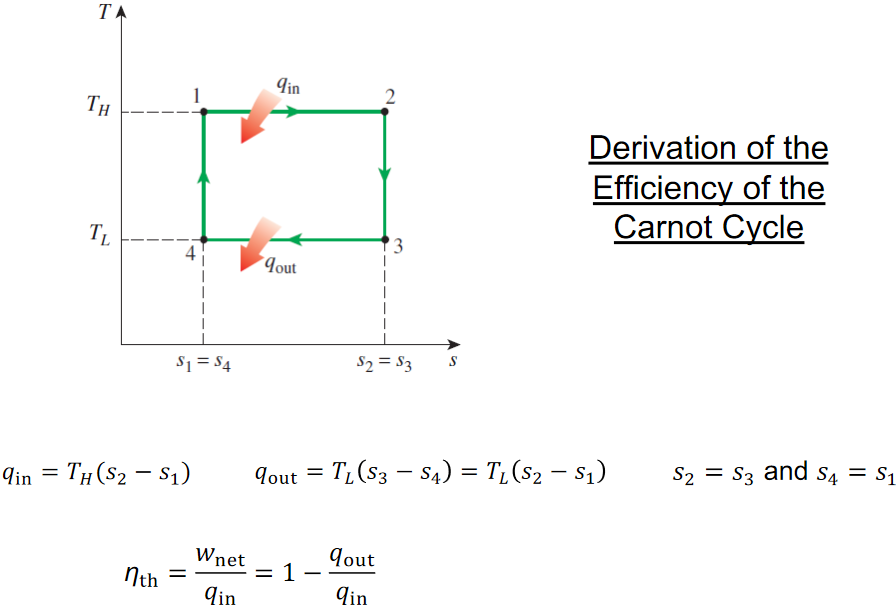
\includegraphics[width=\linewidth]{Images/Carnot_Cucle.png}
    % Air-Standard Assumptions
    \subsection*{Air-Standard Assumptions}
    \begin{itemize}
        \item The working fluid is air which continuously circulates in a closed loop and always behaves as an ideal gas.
        \item All the processses that make up the cycle are internally reversible.
        \item The combustion process is replaced by a haet-addition process from an external source.
        \item The exhaust process is replaced by a heat-rejection process that restores the working fluid to its initial state.
    \end{itemize}
    \textbf{Cold Air Standard Assumptions}: When the working fluid is considered to be air with constant specific heats at room temperature ($25^\circ$C)\par 
    \textbf{Air Standard Cycle}: A cycle for which the air-standard assumptions are applicable.
    % Reciprocating Engines
    \subsection*{Reciprocating Engines}
    \textbf{Compression Ratio}: $r=\frac{V_\text{max}}{V_\text{min}}=\frac{V_\text{BDC}}{V_\text{TDC}}$\par 
    $W_\text{net}=\text{MEP}\times\text{Piston Area}\times\text{Stroke}=\text{MEP}\times\text{Displacement Volume}$\par 
    \textbf{Mean Effective Pressure (MEP)}:\par 
    $\text{MEP}=\frac{W_\text{net}}{V_\text{max}-V_\text{min}}=\frac{w_\text{net}}{v_\text{max}-v_\text{min}}$\par 
    The engine with a larger MEP delivers more work per cycle and thus performs better.\par 
    % The Otto Cycle
    \subsection*{The Otto Cycle}
    The ideal cycle for spark-ignition engines.\par 
    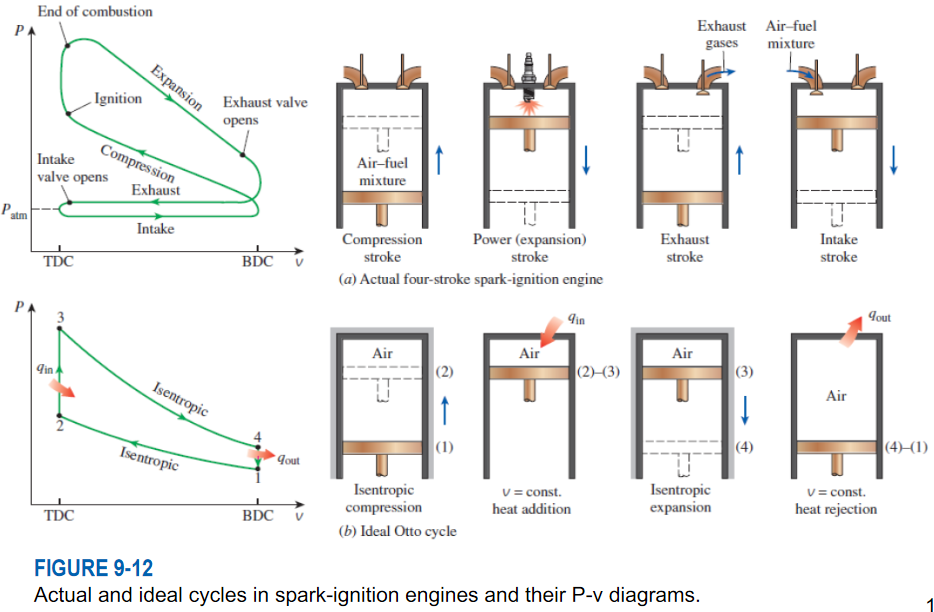
\includegraphics[width=\linewidth]{Images/Otto_Cycle.png}\par
    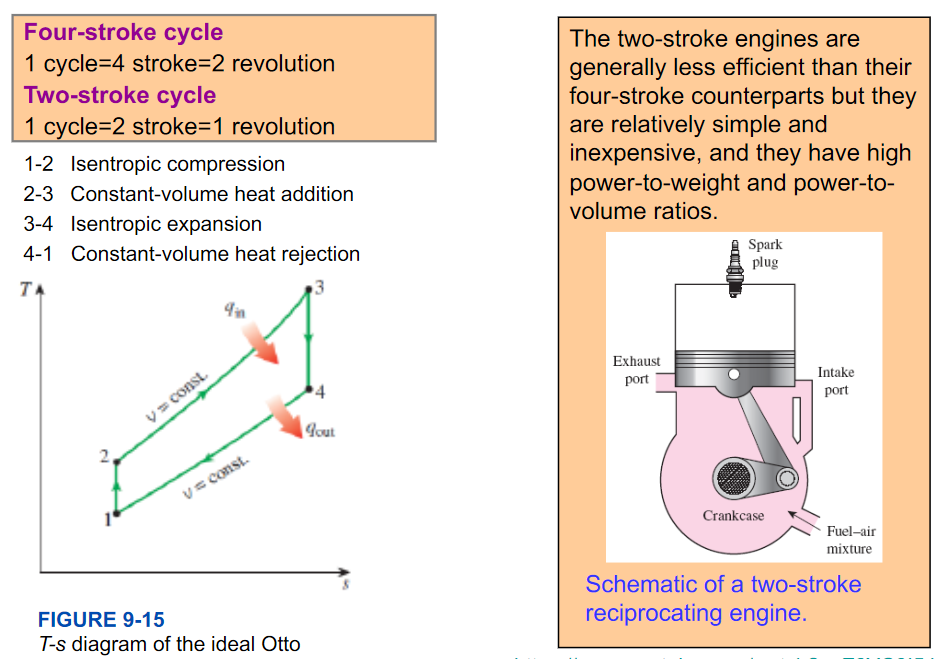
\includegraphics[width=\linewidth]{Images/Otto_Cycle2.png}\par
    For air k=1.4 and the thermal efficiency of the Otto Cycle increases with the specific heat ratio, k, of the working fluid.\par
    $(q_{in}-q_{out})+(w_{in}-w_{out})=u_{exit}-u_{inlet}$\par 
    $q_{in}=u_3-u_2=c_v(T_3-T_2)$\par 
    $q_{out}=u_4-u_1=c_v(T_4-T_1)$\par 
    $\eta_\text{th,Otto}=\frac{w_\text{net}}{q_{in}=1-\frac{q_{out}}{q_{in}}}=1-\frac{T_4-T_1}{T_3-T_2}=1-\frac{T_1(T_4/T_1-1)}{T_2(T_3/T_2-1)}$\par 
    $\frac{T_1}{T_2}=\left(\frac{v_2}{v_1}\right)^{k-1}=\left(\frac{v_3}{v_4}\right)^{k-1}=\frac{T_4}{T_3}$\par 
    $r=\frac{V_\text{max}}{V_\text{min}}=\frac{V_1}{V_2}=\frac{v_1}{v_2}$\par 
    Cold-Air Standard Assumption: $\eta_\text{th,Otto}=1-\frac{1}{r^k-1}$
    % Diesel Cycle
    \subsection*{Diesel Cycle}
    The ideal cycle for the compression-ignition engines.\par 
    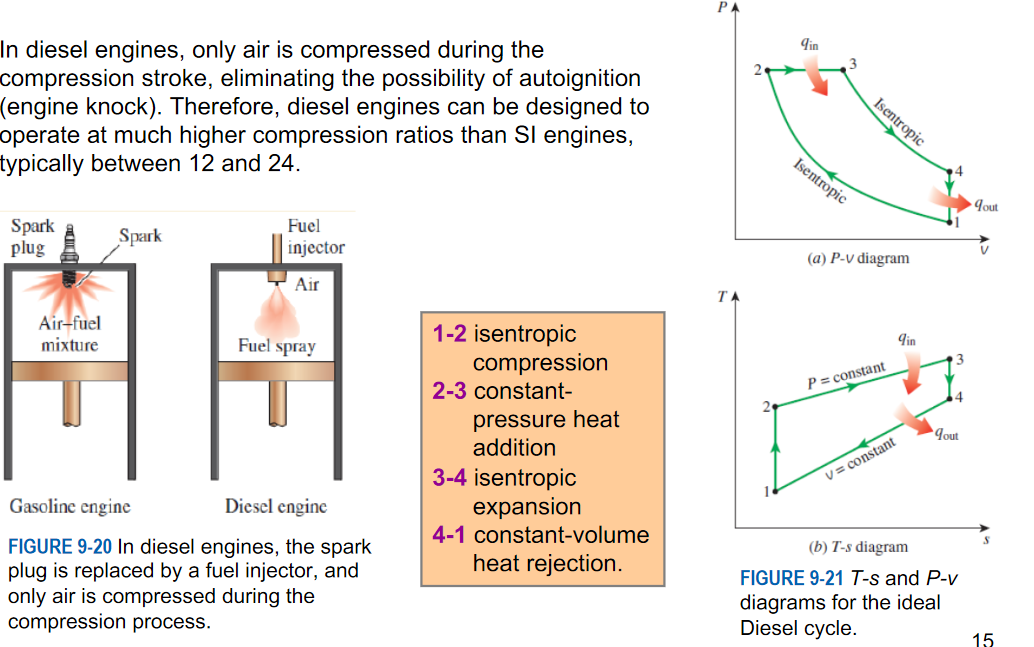
\includegraphics[width=\linewidth]{Images/Diesel_Cycle.png}\par 
    $q_{in}-w_{b,out}=u_3-u_2\rightarrow q_{in}=P_2(v_3-v_2)+(u_3-u_2)=h_3-h_2=c_p(T_3-T_1)$\par 
    $-q_{out}=u_1-u_4\rightarrow q_{out}=u_4-u_1=c_v(T_4-T_1)$\par 
    $\eta_\text{th,Diesel}=\frac{W_{net}}{q_{in}}=1-\frac{q_{out}}{q_{in}}=1-\frac{T_4-T_1}{k(T_3-T_2)}=1-\frac{T_1(T_4/T_1-1)}{kT_2(t_3/T_2-1)}$\par 
    $r_c=\frac{V_3}{V_2}=\frac{v_3}{v_2}$\par 
    $\eta_\text{th,Diesel}=1-\frac{1}{r^{k-1}}\left[\frac{r_c^k-1}{k(r_c-1)}\right]$
    The thermal efficiency of the Diesel Cycle decreases as the cutoff ratio increases and increases as the compression ratio increases.
    % Brayton Cycle
    \subsection*{Brayton Cycle}
    The ideal cycle for gas-turbine engines.\par 
    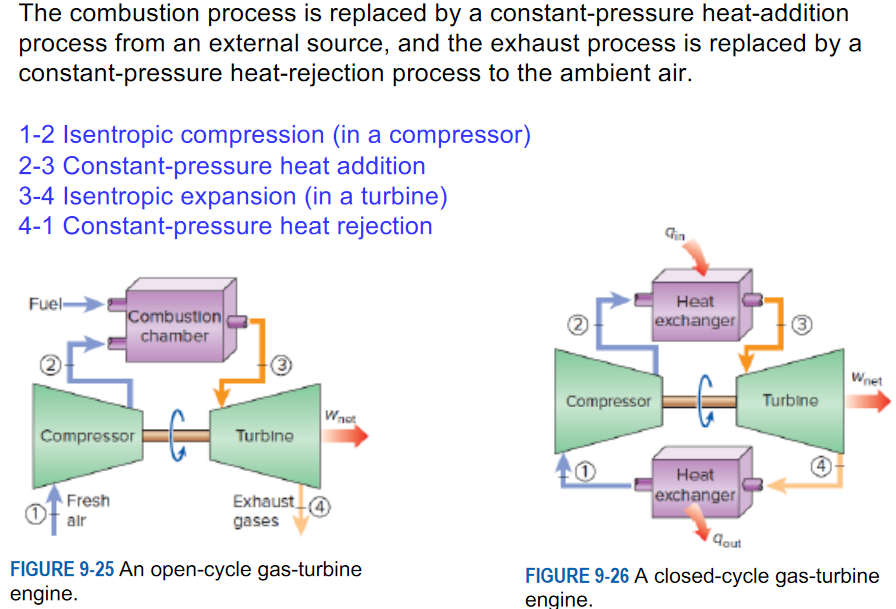
\includegraphics[width=\linewidth]{Images/Brayton.png}\par 
    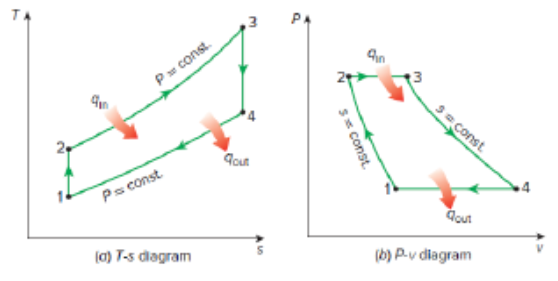
\includegraphics[width=\linewidth]{Images/Brayton2.png}\par 
    The thermal efficiency of the ideal Brayton Cycle increases as the pressure ratio increases.\par
    $(q_{in}-q_{out})+(w_{in}-w_{out})=h_{exit}-h_{inlet}$\par 
    $q_{in}=h_3-h_2=c_p(T_3-T_2)$\par 
    $q_{out}=h_4-h_1=c_p(T_4-T_1)$\par 
    $\eta_\text{th,Brayton}=\frac{w_{net}}{q_{in}}=1-\frac{q_{out}}{q_{in}}=1-\frac{c_p(T_4-T_1)}{c_p(T_3-T_2)}=1-\frac{T_1(T_4/T_1-1)}{T_2(T_3/T_2-1)}$\par 
    $\frac{T_2}{T_1}=\left(\frac{P_2}{P_1}\right)^{(k-1)/k}=\left(\frac{P_3}{P_4}\right)^{(k-1)/k}=\frac{T_3}{T_4}$\par 
    $r_p=\frac{P_2}{P_1}$ Pressure Ratio\par
    Only for ideal cycle and cold-air standard assumptions: $\eta_\text{th,Brayton}=1-\frac{1}{r_p^{(k-1)/k}}$
    % Development of Gas Turbines
    \subsection*{Development of Gas Turbines}
    \begin{itemize}
        \item Increasing the turbine inlet (or firing) temperatures
        \item Increasing the efficiencies of turbomachinery components (turbins, compressors)
        \item Adding modification to the basic cycle (intercooling, regeneration or recuperation, and reheating)
    \end{itemize}
    \textbf{Deviation of Actual Gas-Turbine Cycles from Idealized Ones}:\par
    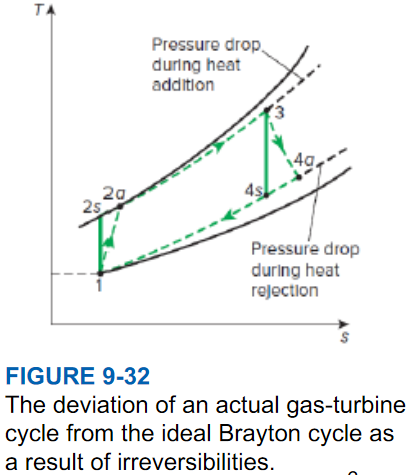
\includegraphics[width=0.5\linewidth]{Images/non_ideal_cycles.png}\par 
    Irreversibilities in turbine and compressors, pressure drops, heat losses.\par 
    Isentropic efficiencies of the compressor and turbine:\par 
    $\eta_C=\frac{w_s}{w_a}=\frac{h_{2s}-h_1}{h_{2a}-h_1}$ and $\eta_T=\frac{w_a}{w_s}=\frac{h_3-h_{4a}}{h_3-h_{4s}}$\par 
    % Brayton Cycle with Regeneration
    \subsection*{Brayton Cycle with Regeneration}
    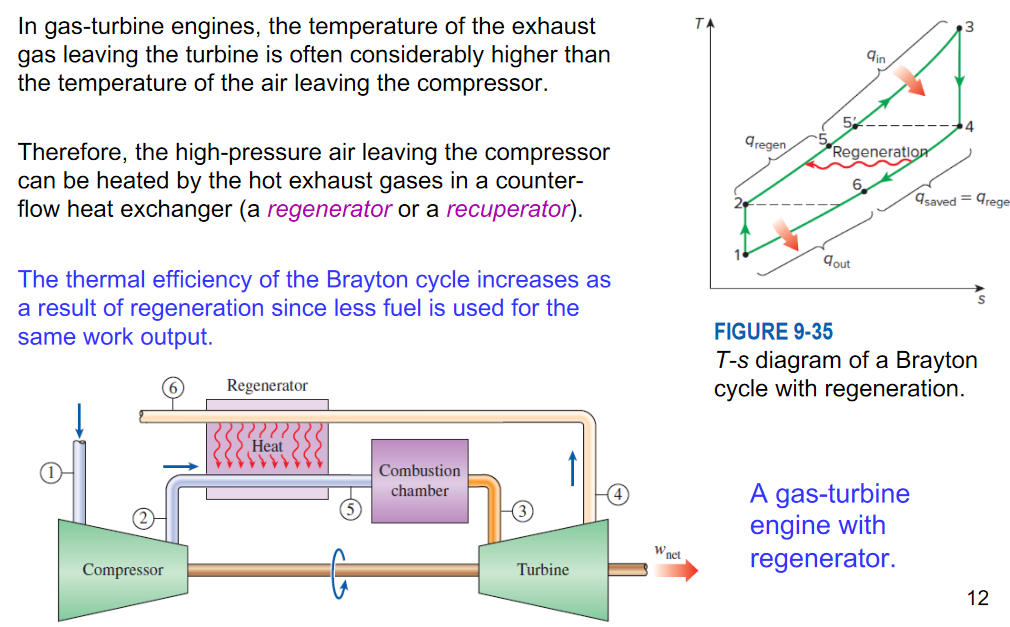
\includegraphics[width=\linewidth]{Images/Brayton_regen.png}\par 
    $q_\text{regen,act}=h_5-h_2$\par 
    $q_\text{regen,max}=h_{5'}-h_2=h_4-h_2$\par 
    Effectiveness of regenerator: $\epsilon=\frac{q_\text{regen,act}}{q_\text{regen,max}}=\frac{h_5-h_2}{h_4-h_2}$\par 
    Effectiveness under cold-air assumptions: $\epsilon=\frac{T_5-T_2}{T_4-T_2}$\par 
    Efficiency under cold-air assumptions:\par $\eta_\text{th,regen}=1-\left(\frac{T_1}{T_3}\right)(r_p)^{(k-1)/k}$\par
    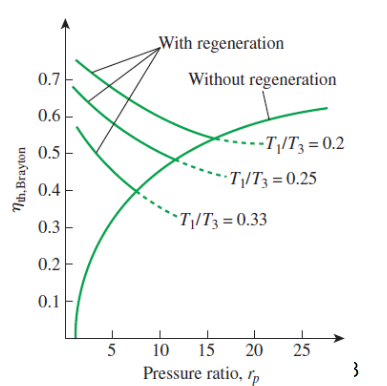
\includegraphics[width=0.5\linewidth]{Images/regen.png}
    % Carnot Vapor Cycle
    \subsection*{Carnot Vapor Cycle}
    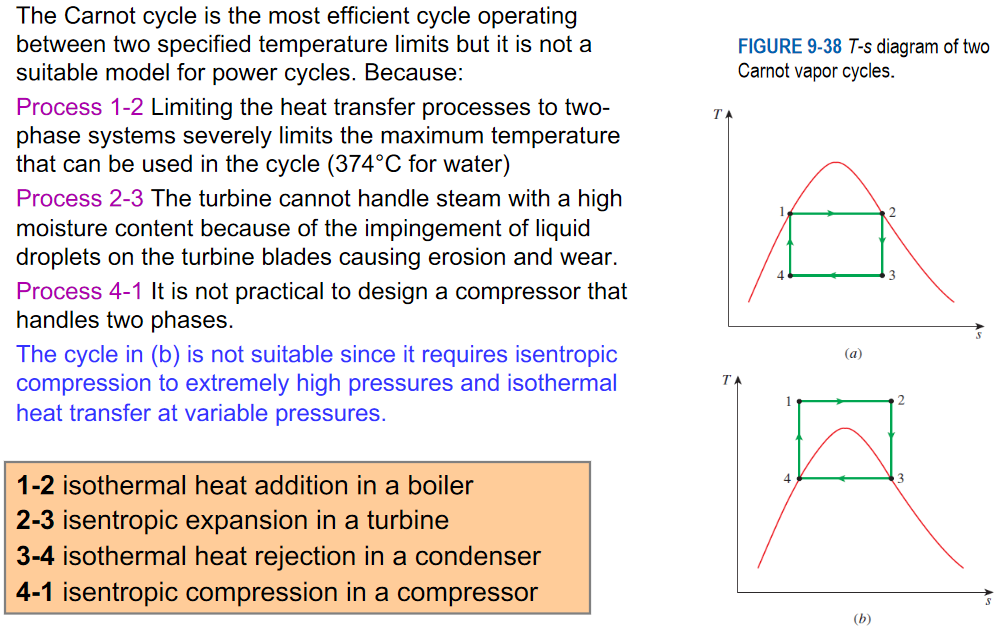
\includegraphics[width=\linewidth]{Images/carnot_vapor.png}
    % Rankine Cycle
    \subsection*{Rankine Cycle}
    The ideal cycle for vapor power cycles.\par
    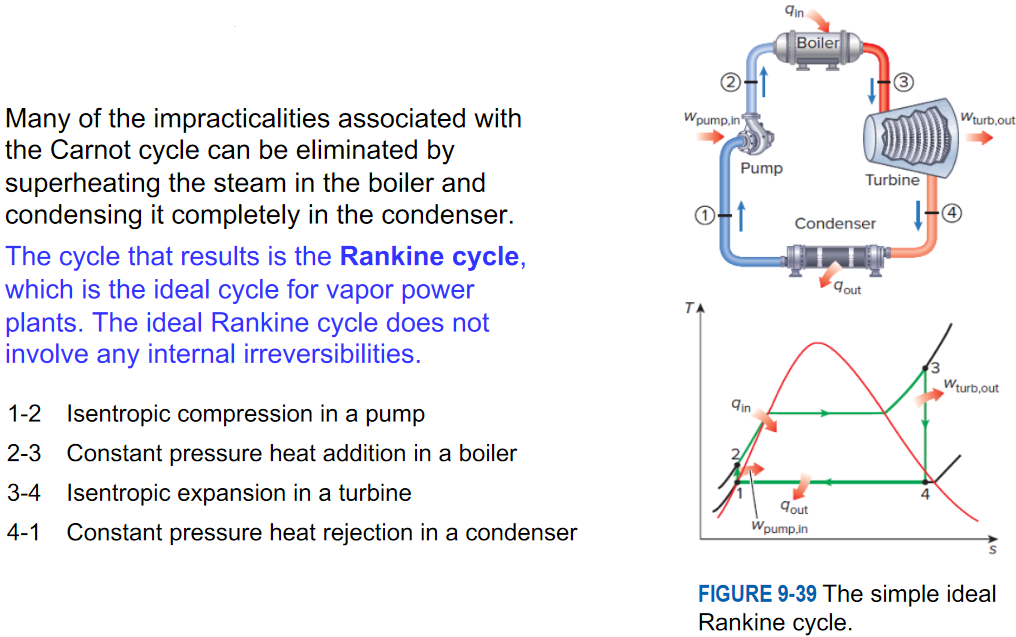
\includegraphics[width=\linewidth]{Images/Rankine_Cycle.png}\par 
    Steady-flow energy equation:\par 
    $(q_{in}-q_{out})+(w_{in}-w_{out})=h_e-h_i$ (kJ/kg)\par 
    \textbf{Pump}(q=0):\par 
    $w_\text{pump,in}=h_2-h_1=V(P_2-P_1)$\par 
    $h_1=h_{f@P_1}$ and $v=v_1=v_{f@P_1}$\par 
    \textbf{Boiler}(w=0):\par $q_{in}=h_3-h_2$\par 
    \textbf{Turbine}(q=0):\par $w_\text{turb,out}=h_3-h_4$\par 
    \textbf{Condenser}(w=0):\par $q_{out}=h_4-h_1$\par 
    \textbf{Finally}:\par 
    $w_{net}=q_{in}-q_{out}=w_\text{turb,out}-w_\text{pump,in}$\par 
    $\eta_{th}=\frac{w_{net}}{q_{in}}=1-\frac{q_{out}}{q_{in}}$\par 
    The efficiency of power plants in the US is often expressed in terms of \textbf{heat rate} which is the amount of heat supplied, in Btu's, to generate 1 kWh of electricity: $\eta_{th}=\frac{3412\text{(Btu/kWh)}}{\text{Heat rate (Btu/kWh)}}$
    % Deviation of Actual Vapor Power Cycle from Idealized Ones
    \subsection*{Deviation of Actual Vapor Power Cycle from Idealized Ones}
    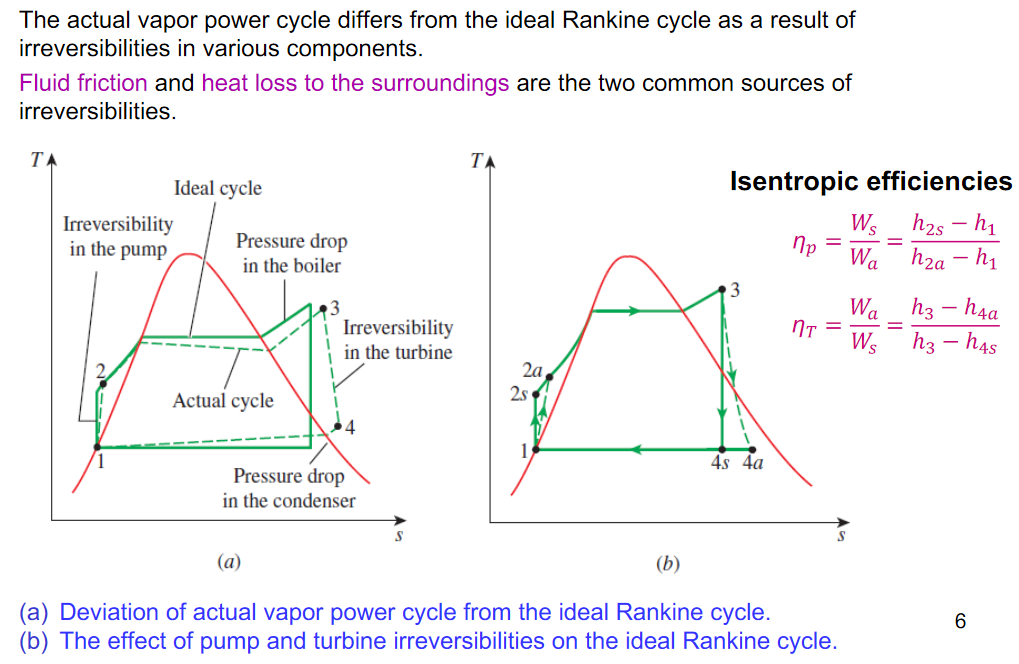
\includegraphics[width=\linewidth]{Images/non_deal_vapor.png}
    % How Increase Efficiency of Rankine Cycle?
    \subsection*{How Increase Efficiency of Rankine Cycle?}
    Look at Lecture 12 starting Page 7 for diagrams.\par
    \textbf{Lowering the Condenser}: Lowers $T_{\text{low,avg}}$, however, it increases the moisture content of the steam at the final stages of the turbine.\par 
    \textbf{Superheating the Steam to High Temperatures}: increases $T_\text{high,avg}$ and decreases the moisture content at the turbine exit (desirable), however it is limited by metallurgical considerations. Highest temp at inlet is 620$^\circ$.\par 
    \textbf{Increasing the Boiler Pressure}: increases $T_\text{high,avg}$ however the moisture content of the steam at the turbine exit increases - can be corrected by reheating the steam.
    % The Ideal Reheat Rankine Cycle
    \subsection*{The Ideal Reheat Rankine Cycle}
    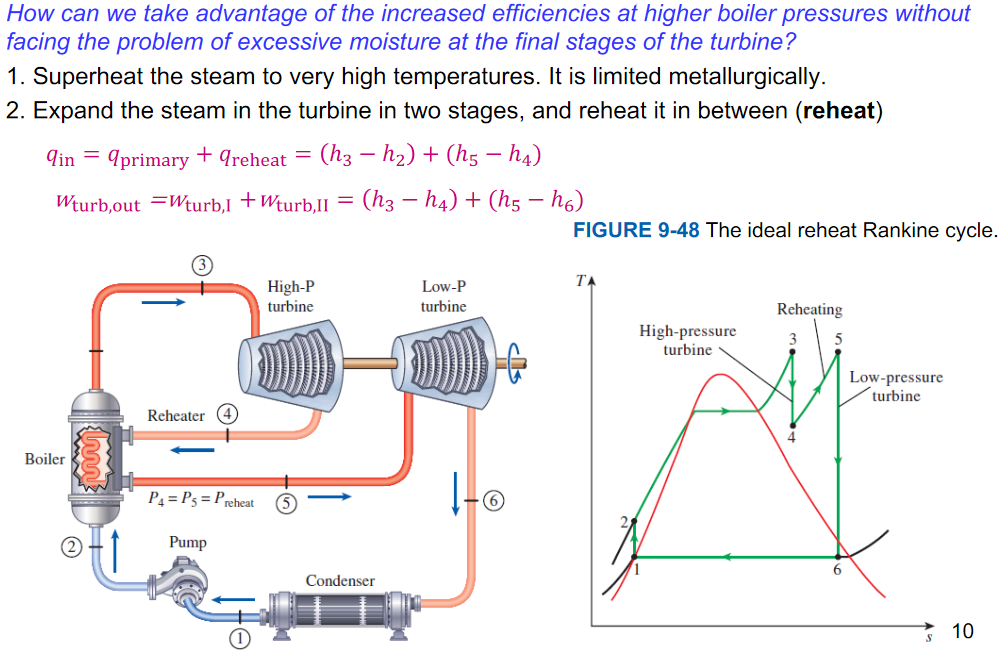
\includegraphics[width=\linewidth]{Images/reheat_rankine.png}
    % Refrigerators and Heat Pumps
    \subsection*{Refrigerators and Heat Pumps}
    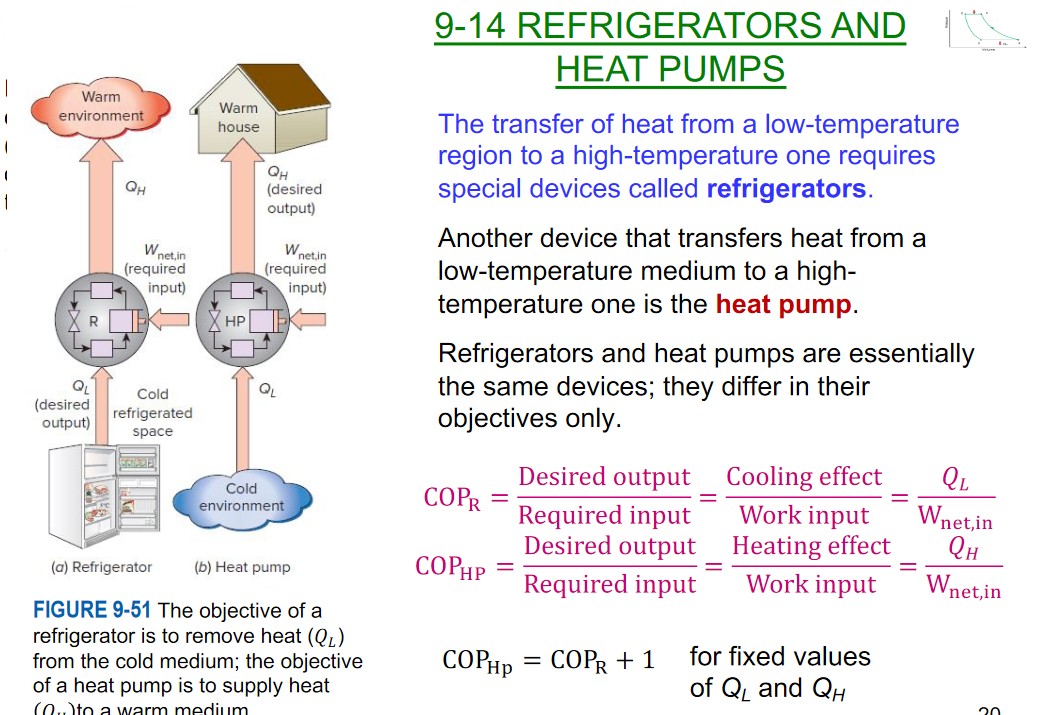
\includegraphics[width=\linewidth]{Images/refrigerators_HP.png}
    % Reversed Carnot Cycle
    \subsection*{Reversed Carnot Cycle}
    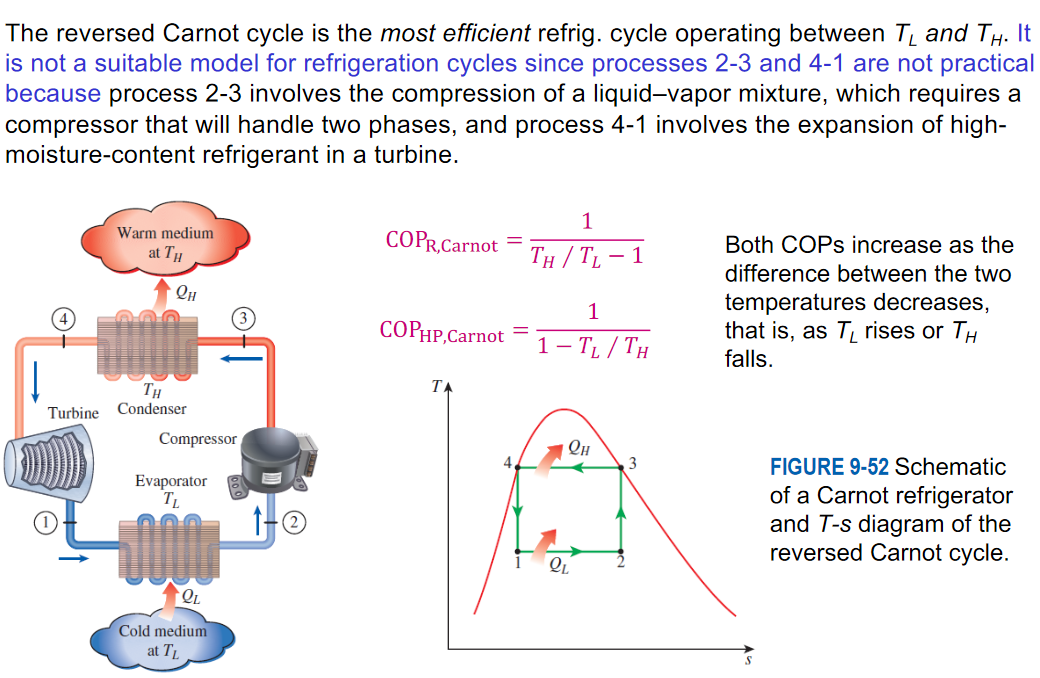
\includegraphics[width=\linewidth]{Images/reverse_carnot.png}
    % Ideal Vapor-Compression Refrigeration Cycle
    \subsection*{Ideal Vapor Compression Refrigeration Cycle}
    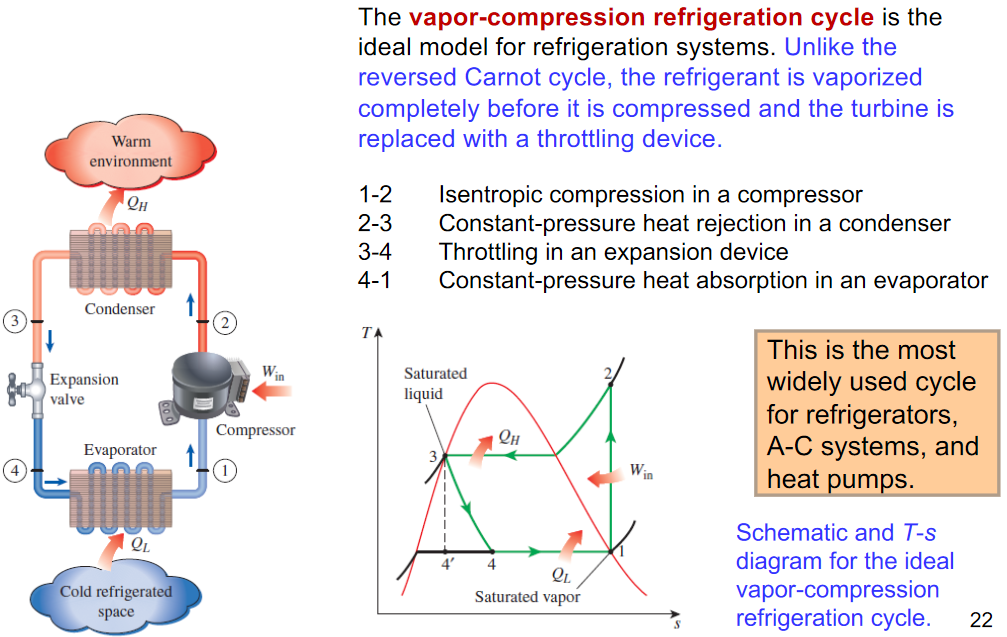
\includegraphics[width=\linewidth]{Images/vcr.png}

    % ----- Mechanisms of Heat Transfer ----- %
    \section*{Mechanisms of Heat Transfer}
    % Conduction
    \subsection*{Conduction}
    The transfer of energy from the more energetic particles of a substance to the adjacent less energetic ones as a result of interactions between the particles.\par 
    Rate of heat conduction $\propto \frac{\text{(Area)(Temperature Difference)}}{\text{Temperature Difference}}$\par 
    $\dot{Q}_\text{cond}=kA\frac{T_1-T_2}{\Delta x}=-kA\frac{\Delta T}{\Delta x}$ (W)\par 
    When $x\rightarrow 0$, $\dot{Q}_\text{cond}=-kA\frac{dT}{dx}$\par 
    \textbf{Thermal Conductivity}: $k$, a measure of the ability of a material to conduct heat.\par 
    \textbf{Temperature Gradient}: $dT/dx$, the slope of the temperature curve on a T-x diagram.
    % Thermal Diffusivity
    \subsection*{Thermal Diffusivity}
    \textbf{Specific Heat}: $c_p$ (J/kgC), heat capacity per unit mass.\par 
    \textbf{Heat Capacity}: $\rho c_p$ (J/m$^3$), heat capacity per unit volume.\par 
    \textbf{Thermal Diffusivity}: $\alpha$ (m$^2$/s), represents how fast heat diffuses through a material.\par 
    $\alpha = \frac{\text{Heat Conduction}}{\text{Heat Storage}}=\frac{k}{\rho c_p}$\par 
    The larger the thermal diffusivity the faster the propogation of heat into the medium.
    % Convection
    \subsection*{Convection}
    The mode of energy transfer between a solid surface and the adjacent liquid or gas that is in motion, and it involves the combined effects of conduction and fluid motion.\par 
    $\dot{Q}_\text{conv}=hA_s(T_2-T_\infty)$ where $h$ is the convection heat transfer coefficient in W/m$^2$K
    % Radiation
    \subsection*{Radiation}
    The energy emitted by matter in the form of electromagnetic waves as a result of the changes in the electronic configurations of the atoms or molecules.\par 
    $\dot{Q}_\text{emit,max}=\sigma A_sT_s^4$ where $\sigma = 5.670\times 10^{-8}$ W/m$^2$K$^4$ or $0.1714\times 10^{-8}$ Btu/hft$^2$R$^4$\par 
    The idealized surface that emits radiation at this maximum rate is called a blackbody. The radiation for all real surfaces is as:\par 
    $\dot{Q}_\text{emit}=\varepsilon\sigma A_2T_s^4$ (W) where $\varepsilon$ is the emissivity of the surface. $\alpha$ is the absorptivity of the surface.\par 
    $\dot{Q}_\text{absorbed}=\alpha\dot{Q}_\text{incident}$\par 
    $\dot{Q}_\text{rad}=\varepsilon\sigma A_s(Ts^4-T_\text{surr}^4)$ (W)\par 
    Convection and Radiation often take place in parallel:\par 
    $\dot{Q}_\text{total}=\dot{Q}_\text{conv}+\dot{Q}_\text{rad}=h_\text{combined}A_s(T_s-T_\infty)$\par 
    $h_\text{combined}=h_\text{conv}+h_\text{rad}=h_\text{conv}+\varepsilon\sigma(T_s+T_\text{surr})(T_s^2+T_\text{surr}^2)$

    % ----- General Knowledge ----- %
    \section*{General Knowledge}
    \textbf{Isentropic}: Constant entropy\par 
    \textbf{Isothermal}: Constant temperature\par 
    \textbf{Adiabatic}: No Q\par 
    \textbf{Adiabatic and Reversible}: Isentropic\par


\end{multicols}  
\end{document}